
 \section{kagu}


\subsubsection*{ kagu framework architecture
}

 kagu uses  both containers (Docker) and virtual machines (libvirt/kvm/qemu).  Libvirt is used to create long-lived topologies whose members are test agents, test targets and the virtual network links which integrate the distinct VMs into a single connected system.  The motivation for this high level design is to provide a controlled and configurable execution environment for virtual routers and test agents.  The system is designed to enable moderately large networks containing interlinked multiple test targets and test agents, such as is required to validate system level behaviour in multi-AS BGP networks.  Hardware virtualisation is required because the representative commercial grade BGP systems are provided as VM images, and are not based on Linux operating system. `
 `
 % One of the kagu subsystems is responsible for building these topologies, including the automatic generation of mesh topologies, and another kagu component, a guest VM agent, enables auto discovery of virtual neighbour addresses and interfaces without explicit, per guest node, configuration.  This is otherwise non-trivial when all the inter-VM links are point to point, so that no system level address autoconfiguration scheme (e.g. DHCP) is available, and in fact in data centre BGP implementations there are extensions to BGP to support just these capabilities.  Unfortunately, these extensions are not applicable to this test environment, and are not supported in the software of most of the BGP systems in the list of targets.  `
Whilst this design achieved the goal of delivering a suitable hardware infrastructure it complicates the test orchestration task, even without considering the issues of exception management.  In the initial kagu design the approach adopted was to use remote ssh shells to monitor and execute every aspect of the tests, however this proved to be both unreliable and extremely complex to build.  The eventual solution is simpler, more reliable and more capable and flexible \- the solution adopted is ‘remote docker’.  This approach builds a single standardised VM container which can be used for all test targets, test agents, and all distinct nodes in a test constellation. Nodes are configured by role using different docker images, and configured for node specific identity by configuration files injected into docker instances.  Finally, the problem of collecting exception context is solved by a combination of Docker’s  internal logging via systemd/journald, and the innovation of defining core-dump destinations as files mounted *outside* the docker container.  In this way, each Docker instance can be managed as a single logical object which may be stopped on command, or exit unexpectedly, with error status, yet whose exception logs are reliably persisted in a central location, independent of the execution environment.  The critical capability provided by Docker is the facility to control *and log* Docker daemons on remote servers from a remote single separate control node. `

Implementation note: in all cases Docker instances are run in a privileged mode in the host VM, in order to allow the running BGP speaker to have direct access to all network interfaces; the reason that Docker alone is not sufficient itself for this application is that although Docker can be used to restrict guest processor and memory allocation it was not found possible to manage the virtualised network topology using Docker in the way that is possible with libvirt/kvm, and secondly, some test target are not available for native Docker use since they are provided as KVM VMs.

% #### ‘testscripts’

% ‘testscripts’ refers to the interactive, tmux based, alternative to ‘kagu’.  Functional test don’t require repeated lengthy execution, but they do require immediate in depth visbility of routing response after different stimuli.

% #### testscript deployment and uses cases

% # Bootstrapping a test environment: full instructions

% The target environment is a current Linux distribution system capable of running qemu/kvm virtualised hosts.  A medium-spec laptop or desktop is required \- the limiting factor is RAM and virtualisation capable CPU \- an 8GB machine has been used successfully.
\NH{need to pull in here the BGP protection test setup}

% \section{PIR test implementation guide}

\NH{\rule{14cm}{0.4pt}}

\NH{this text is to be relocated in the kagu section}


\subsection{functional components of PIR test environment}

\subsubsection{server, OS, virtualisation host}

The current server and OS are Ubuntu Linux 22.04 (laptop) and Ubuntu Linux 20.04 (rack mount server).
Laptop has 32 GB RAM and 14 CPU cores (Intel i7-1280P), server 128GB RAM, 20 CPU cores (Intel Xeon D-1747NTE).

Virtualisation support is standard Linux KVM/qemu managed with libvirt.
Container technology is standard Docker.

\subsection{virtual routers, software routers}
\subsubsection{versions}

\begin{enumerate}
\item Cisco virtual router: IOSv - VIOS-ADVENTERPRISEK9-M - Version 15.7(3)M3
\item Juniper virtual router: Junos VMX - JUNOS 18.2R1.9
\item Bird.cz - BIRD2 - version 2.15.1
\item frr - version 8.4.4 (installed via package manager in ubuntu24.04)
\item OpenBGPD - version 8.6
\item gobgp - version 3.35.0
\end{enumerate}

\subsubsection{build procedures - Docker images}

\begin{enumerate}
\item Bird2 and OpenBGPD are built from source
\item frr is installed as an ubuntu package
\item gobgp is installed as a binary from OSRGs github repository.
\end{enumerate}

\subsubsection{build procedures - virtual router images}

\begin{enumerate}
\item <reference source file directory>
\end{enumerate}

A custom configuration tool was developed for both Cisco and Juniper as an 'expect' script which drivers a clean router instance by invoking command line scripts which copy in the configuration files based on the router role requested.  The configuration files consist of 'standard' IOS and Junos configuration CLI commands.
The scripts allow many full router configurations to be maintained and updated and used on demand to (re-)create the desired set of routers for an experiment.

A virtual router is built from a suitable 'qcow2' image using the 'virt-install' tool and nominating the OS variant as freebsd12.0'.

Junos images are assigned 4Gb RAM and use 'virtio' network drivers.

Cisco images are assigned 2Gb RAM and use 'e1000' network drivers.

The virtual image builder is developed under the project heading 'kagu'.


\NH{\rule{14cm}{0.4pt}}

\section{`Smoketest'}

\subsection*{What is smoketest?}
'smoketest' is the core test \textit{framework} (\textit{kakapo} is the core test BGP speaker).

\begin{figure}[H]
    \centering
    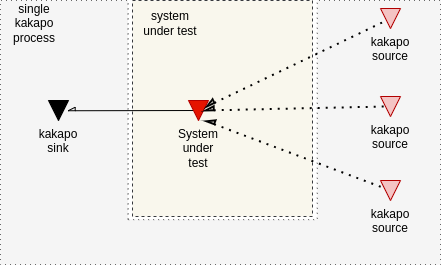
\includegraphics[width=0.7\linewidth]{images/bgp6.drawio.png}
    \caption{standard kakapo test deployment configuration}
    \label{fig:diag6}
\end{figure}

It orchestrates concurrent instances of a wide range of target test BGP systems and the BGP test system, `kakapo'.

In general, most of the test BGP systems are run under the control of Docker\footnote{Cisco vIOS and Juniper vMX are run as full virtual machines under KVM}.

The test procedures orchestrated by smoketest are all variants on a `standard' kakapo configuration\footnote{The following description is best understood after reading about kakapo in the previous section.}, i.e., kakapo emulates two or more BGP endpoints to act as BGP route sources of sinks, all of which are configured as direct peers to the single System-Under-Test.
Kakapo route-source endpoints announce new routes according to some pre-defined pattern, and a singleton kakapo route-sink monitors the relayed routes as they are re-announced by the System-Under-Test (SUT).


\section{kagu - alt 1}


\subsection{Kagu: BGP experiment automation}

A major challenge for network experimentation is reproducibility. Kagu is an
automation platform, built around kakapo, allowing experimenters to deploy and
parallelise the execution of BGP experiments. In parallel, kagu also automates
measurement data and logging information collection for offline processing.

OS virtualisation is a key technological enabler for Kagu, which supports
integration with docker and the libvirt management library.  The docker
integration allows kagu to run kakapo and software router as docker containers
and to use docker management operations to spawn and terminate them.
Furthermore, detailed logging information are collected through the
systemd/journald services in the container. In order to run an experiment, the
platform requires as input the router and the kakapo configuration parameters
and the platform will use docker technologies to execute the experiment and
collect the results.

Furthermore, libvirt integration allows kagu to deploy large-scale experiments
with complex network topologies over a hypervisor-based virtualisation
platform, like KVM. VMs derive from a base Ubuntu image with the dockerd
daemon installed and configured to exposes remote access via HTTP.

During the deployment of a multi-host experiment, kagu builds all the required
virtual links between VMs, as well as a control plane network which uses
dynamic DNS and cloud-init to map VM control interface addresses to user
friendly host names. A custom libvirt network topology provisions distinct
unique virtual network address blocks onto each VM and dynamically updates the
configuration of a local DNS server.  Finally, the framework offers an
arp-router agent which install routes to loopback and allows connectivity over
unnumbered network interfaces.

Both test harness (kakapo) and target systems are bundled as Docker images
which enables them to be easily started and stopped in remote virtual machines
using the ‘remote Docker’ feature.  Remote Docker allows standard Docker
commands, such as ‘docker run’, ‘docker kill’ and ‘docker pull’ to be executed
on arbitrary target systems from a single controlling machine  Thus a cluster
of multiple VMs having varying resource capability can easily be orchestrated
to run multiple sets of experiments in parallel.  A complementary set of
scripts (kakapo-virt) is used to create and provision the target virtual
machines.

The main system elements are:

\begin{itemize}
	\item kakapo core  a ‘C’ language BGP test tool which can act
	      as a BGP peer, operating simultaneously in both route sink and route source
	      modes
	\item kakapo relay  a ‘dummy’,‘C’ language, BGP router which allows
	      baseline calibration of the test system
	\item kakapo runner  a run-time
	      integration framework for controlling multiple test runs with ranges of
	      test parameters
	\item kakapo ingest  offline analysis of the test data
	      generated by kakapo, including on-demand gnuplot graph display
	\item
	      kakapo-virt  a VM and virtual network provisioning tool --- kakapo virt
	      creates and provisions test VMs with different resources (CPUs, RAM,..) to
	      provide execution environments for kakapo targets and test harness instance
	      to execute in.  Kakapo-virt also provisions both a control plane network to
	      allow remote orchestration of the VMs and their Docker execution
	      environment, and a separate experimental network context which meshed VMs
	      which are configured to operate as a single experimental topology
	      somewhat like mininet, but for KVM virtual machines.

	\item kagu a build and deploy system for the (mostly Dockerised) components of kakapo
	\item arproute a network utility which enables virtualised systems to discover routes between themselves without manual configuration.
	\item Docker, systemd, libvirt and nginx with webdav support --- provides the infrastructure environment in which kagu and kakapo operate
\end{itemize}

Of these components some work before a testing session (kagu, kakapo-virt), and
others after testing sessions have finished (kakapo ingest).  The core system
consists of kakapo core, kakapo relay, kakapo runner: of these kakapo runner
is the coordination tool: it schedules execution of test systems in virtual
environments, typically systems consisting of kakapo core paired with another
BGP speaker such as bird, frr (quagga), OpenBGP, hbgp, or another hardware or
software router.  Kakapo core starts and stops BGP peer sessions with the
SystemUnderTest, monitors the response performance and records the
configuration and results in test data files on a centralised storage system
for later analysis.  Kakapo runner feeds the required test parameters to kakapo
core: typically these specify a range of BGP route table sizes (two
parameters), and a cycle count for the number of repetitions of route changes
to send, updating the initial route table load.  The recorded results are delta
time measurements for the begin and end of both reception and transmission of
groups of Update messages.  Results are uploaded as structured text files to
a webdav server.

% % \subsubsection{Docker usage}

% % \subsubsection{kakapo-core}

% % \subsubsection{kakapo-relay}

% % \subsubsection{Linux TCP / kernel limitations}

% % Observations of the network behaviour of both the existing platforms such as
% % frr, bird and OpenBGP, and also the custom implementations developed for the
% % study (hbgp, kakapo and kakapo-relay) show the impact of Linux TCP
% % implementations and default configuration

% \subsubsection{Data analysis --- kakapo-ingest}

% Kakapo-ingest is an offline tool which consumes the output generated by
% kakapo-core.  Kakapo currently uses webdav as a repository access mechanism: at
% the end of every execution of a single kakapo run a text based data file is
% uploaded to a central server using webdav.  The file format captures ‘metadata’
% such as the kakapo parameters defining RIB size, update blocking factors,
% prefixes per update, as well as all significant context for the experiment,
% e..g the software router name and version, the number of cores and RAM
% allocation, the date and time of the experiment, and the ‘topic’ which is used
% to group a group of experiments which collectively define an entire
% ‘experiment’

% Kakapo-ingest is a tool whose purpose is to select and preprocess the raw data
% from multiple kakapo-core runs into a format suitable for graph plotting or
% further analysis.  K-ingest resembles an SQL query tool in that it requires
% a set of selection terms to be given which represent a filter over the total
% set of data points.  The Query syntax allows an explicit selection of
% a ‘x-axis’ variable and a separate discrete multi-line selector value set,
% combined with filter terms which define specific values which must match data
% points in order to include them.

% In operation Kakapo-ingest takes a directory path (/var/webdav in the example
% below), and recursively scans it for data files in the correct kakapo format.
% Kakapo-ingest has several modes of execution which allows the dataset to be
% queried and selection criteria defined up to the point that a coherent set of
% data points can be extracted and plotted in a gnuplot graphing environment.

% An example k-ingest query is:

% ingest /var/webdav TOPIC=RIBTEST PLATFORM=bird,frr,bgpd,hbgp RIBSIZE=?

% % In this example, a graph is defined using the metadata field ‘RIBSIZE’ as the
% control parameter (y-axis), and showing separate plots for each of the named
% platforms (bird, frr, OpenBGP, haskell BGP).  In this case there were no
% variants such as CPU count or RAM size present in the database, and so the
% query is already unambiguous and able to directly generate a gnuplot data file
% and if required plot it interactively or export to a graphic file.  Otherwise
% additional selection terms would be required, such as

% ingest \ldots CORES=4 MEMORY=8192

% The flexible query syntax enables other parameters to be plotted, for example
% a graph showing performance for different numbers of prefixes in a fixed count
% of Updates is possible simply by changing the control parameter to ‘GROUPSIZE’
% and defining a suitable range of parameters in kakapo-runner to create the
% required dataset.
